\documentclass{beamer}

\usepackage{amsmath,amssymb,amsthm,graphicx}
\usepackage{caption,subcaption}
\usetheme{Copenhagen}
 \newcommand{\N}{\mathbb{N}}
 \newcommand{\Z}{\mathbb{Z}}
 \newcommand{\Q}{\mathbb{Q}}
 \newcommand{\R}{\mathbb{R}}
 \newcommand{\C}{\mathbb{C}}
 \newcommand{\bM}{\begin{bmatrix}}
 \newcommand{\eM}{\end{bmatrix}}
 \newcommand{\Ni}{\N\cup\{\infty\}}
  \newcommand{\rmD}[1]{\mathrm{d}#1}
\newcommand{\floor}[1]{\lfloor #1 \rfloor}
\title{Optimal Path Planning for Robotic Arms in Household Assistance}
\author{Vikram Sunder and Zachary Greenberg}

\begin{document}
\begin{frame}
\maketitle
\end{frame}

\section{Introduction}
\begin{frame}{The Robot}
\begin{itemize}
\item Irobot Create Base\\
\item 5-degree of freedom arm
\end{itemize}
\begin{figure}[htb]
\centering
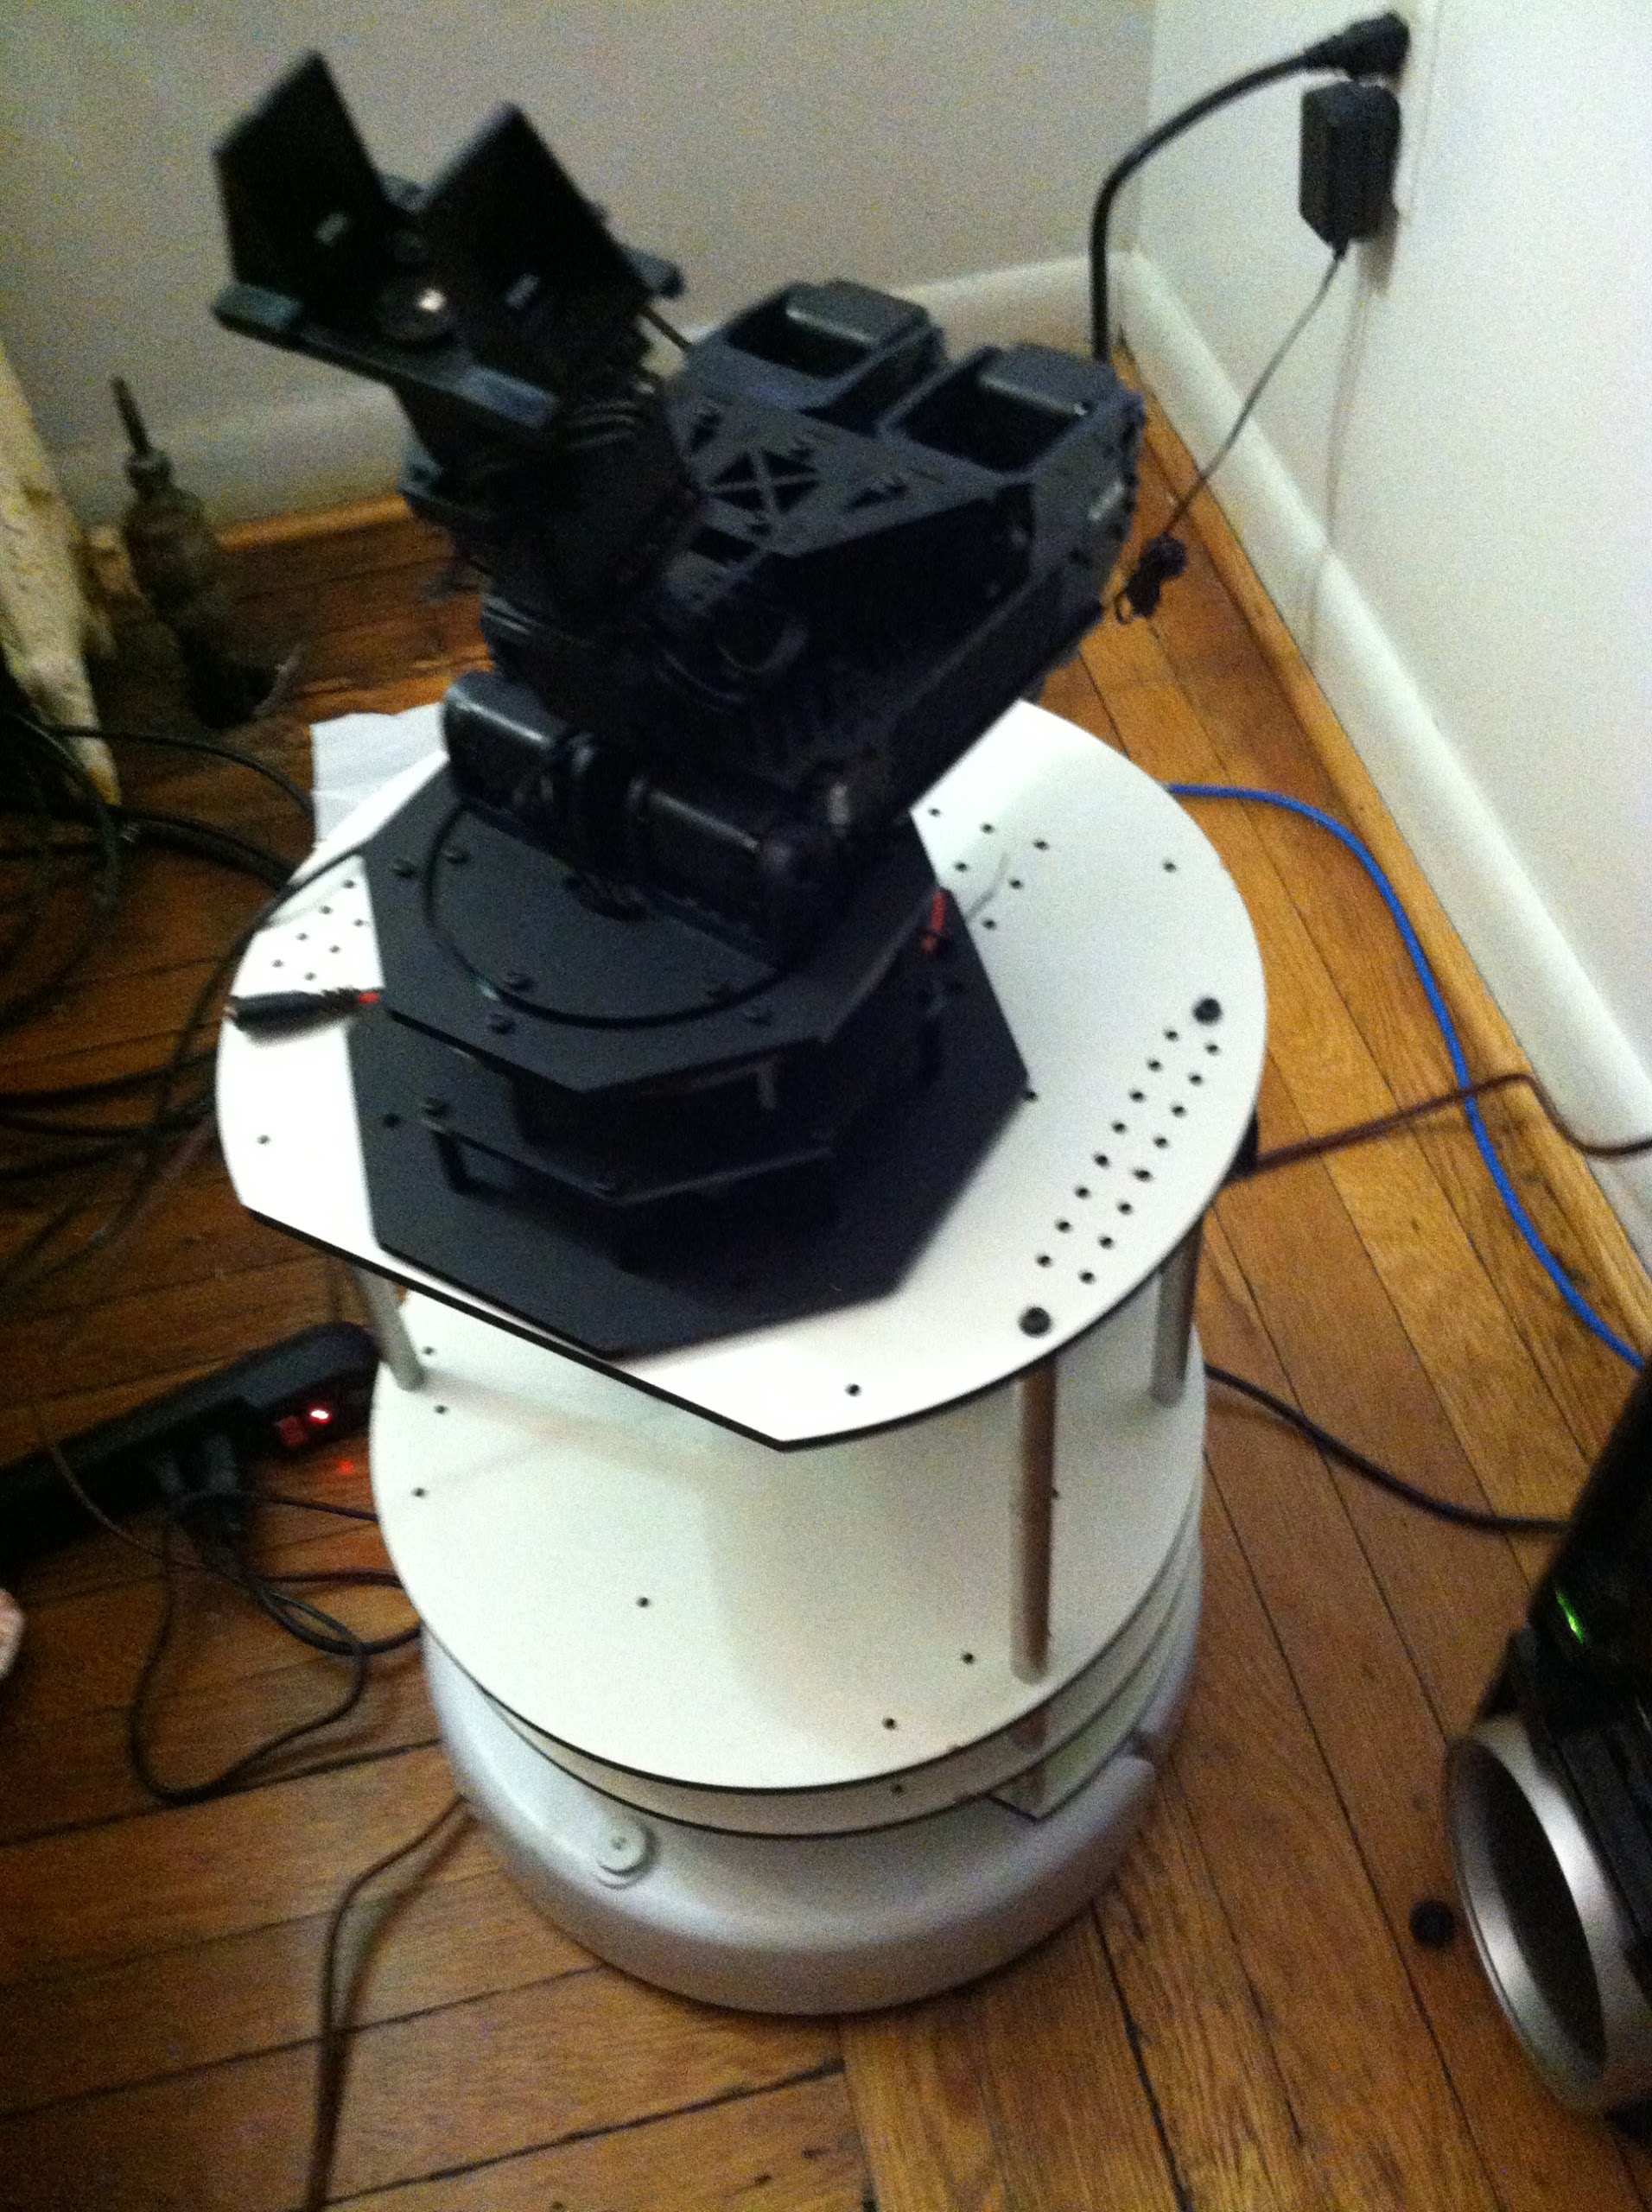
\includegraphics[scale=.05]{PathPics/Robot_With_Arm.jpg}
\end{figure}
\end{frame}

\begin{frame}{The Problem}
Find the shortest path the arm should take to a point.\\
~\\
Explore different notions of ``shortest'' to get different paths.
\begin{itemize}
\item Euclidean Distance
\item Energy Required to Hold an Object
\item Kinetic Energy
\end{itemize}
\end{frame}
\begin{frame}{The Algorithm}
\begin{itemize}
\item Divide configuration space into a grid to make a graph.
\item We used $A^*$ to compute the shortest path in the graph.
\item Use different cost functions to simulate different metrics.
\item As long as the cost is at least the euclidean distance, then the euclidean distance to the target is an admissible heuristic.
\end{itemize}
\end{frame}
\begin{frame}{Kinematics}
Forward Kinematics is a mapping $FK$ from configuration space to work space.\\
The Jacobian $J$ is the derrivitave matrix for $FK$.\\
To get linear velocities from angular velocities $\dot{\theta}$ take $J\dot{\theta}$\\
The $J^T$ maps from workspace forces to torques. $\tau = J^TF$.\\
~\\
For our robot only the first 4 angles determine position.\\
In addition the first angle determines the plane the arm moves in. So we can solve for it first and only have to search 3 dimensional space for the path.
\end{frame}

\section{Results}
\begin{frame}{Euclidean Distance}
Compute distance between nodes in work space.\\
Considering the angle of the end effector gives a different path.
\begin{figure}[htb]
\centering
\begin{subfigure}[b]{0.5\textwidth}
\centering
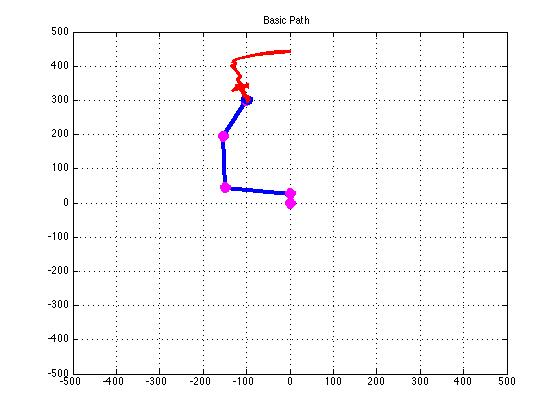
\includegraphics[scale=.3]{PathPics/Basic_Path.jpg}
\caption{Orientation Path}
\end{subfigure}%
~ 
\begin{subfigure}[b]{0.5\textwidth}
\centering
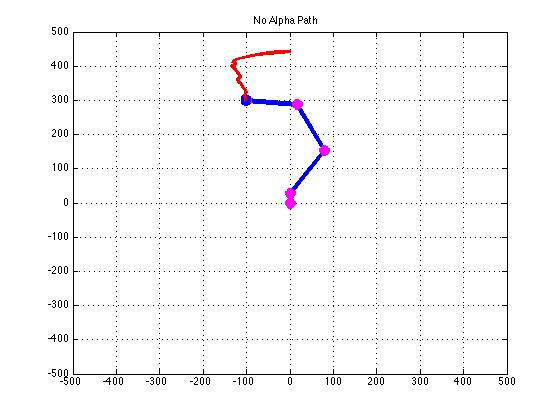
\includegraphics[scale=.3]{PathPics/NoAlpha_Path.jpg}
\caption{No Orientation Path}
\end{subfigure}

\caption{Euclidean Distance Paths}
\label{fig:basicPaths}
\end{figure} 

\end{frame}

\begin{frame}{Energy To Hold Up an Object (Next State)}
Add the energy to hold up an object of weight $m$ in the next state:\\ 
$$	d(u,v) =  \left\|(FK(u)-FK(v))\right\|^2 + \small\left\|J^T_v\bM 0 \\ 0 \\ mg \eM\right\|^2$$\normalsize
\begin{figure}[htb]
\centering
\begin{subfigure}[b]{0.5\textwidth}
\centering
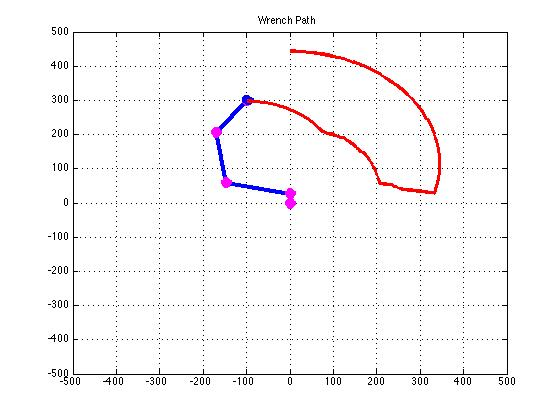
\includegraphics[scale=.2]{PathPics/Wrench_Path.jpg}
\caption{Orientation Path}
\end{subfigure}%
~ 
\begin{subfigure}[b]{0.5\textwidth}
\centering
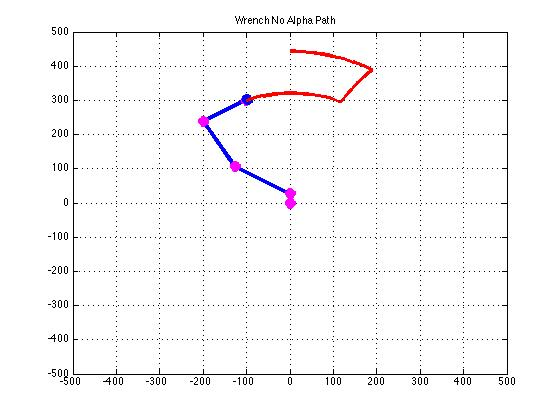
\includegraphics[scale=.2]{PathPics/Wrench_NoAlpha_Path.jpg}
\caption{No Orientation Path}
\end{subfigure}

\caption{Paths When Considering Energy To Hold Up an Object}
\label{fig:EnergyPaths1}
\end{figure}
\end{frame}

\begin{frame}{Energy to Hold Up an Object (Ratios)}
Using the ratio of torques between the states gives:
 $$	d(u,v) =  \left\|(FK(u)-FK(v))\right\|^2 + \Tiny\frac{\left\|J^T_v\bM 0 \\ 0 \\ mg \eM\right\|^2}{\left\|J^T_u\bM 0 \\ 0 \\ mg \eM\right\|^2}$$\normalsize
\begin{figure}[htb]
\centering
\begin{subfigure}[b]{0.5\textwidth}
\centering
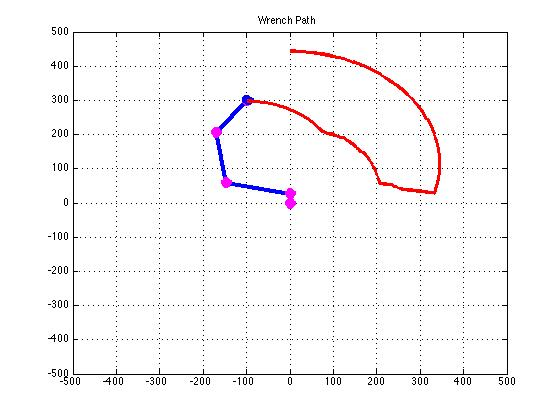
\includegraphics[scale=.19]{PathPics/Wrench_Path.jpg}
\caption{Path When Only Considering The Next State}
\end{subfigure}%
~ 
\begin{subfigure}[b]{0.5\textwidth}
\centering
%\includegraphics[scale=.19]{PathPics/Bad.jpg}
\caption{Path for Ratio of Torques}
\end{subfigure}

\caption{Paths When Considering Energy To Hold Up an Object}
\label{fig:EnergyPaths2}
\end{figure}
\end{frame}
\begin{frame}{Kinetic Energy}
Let $J$ be the Jacobian. Let $\dot{\theta}$ be the angular velocity vector.
 \small\[E_{linear} = \frac{1}{2}m \|J_u\dot{\theta}\|^2\]. \\
\[E_{angular} = \frac{1}{2}m \left\|\frac{\Delta\theta_1+\Delta\theta_2+\Delta\theta_3)}{h}\right\|^2\]\normalsize
\begin{figure}[htb]
\centering
\begin{subfigure}[b]{0.33\textwidth}
\centering
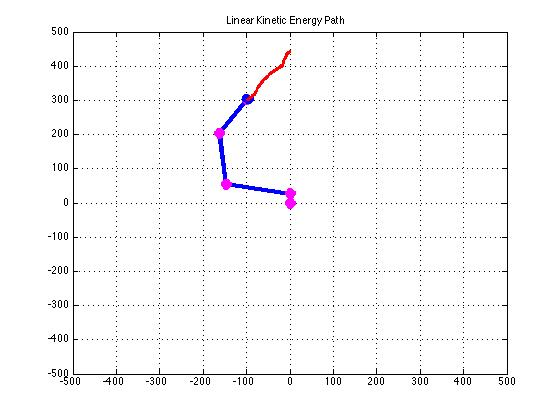
\includegraphics[scale=.135]{PathPics/Energy_Linear_Path.jpg}
\caption{Linear Kinetic Engery Path}
\end{subfigure}%
~ 
\begin{subfigure}[b]{0.33\textwidth}
\centering
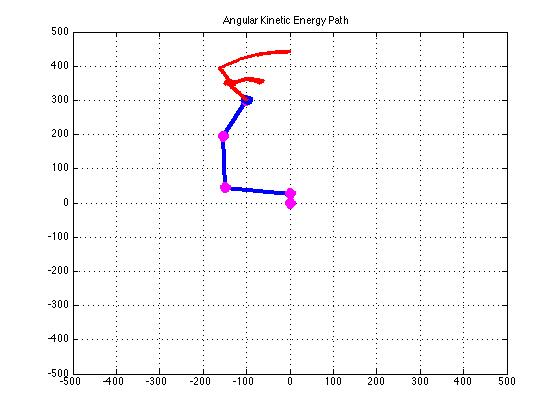
\includegraphics[scale=.135]{PathPics/Energy_Angular_Path.jpg}
\caption{Angular Kinetic Energy Path}
\end{subfigure}%
~ 
\begin{subfigure}[b]{0.33\textwidth}
\centering
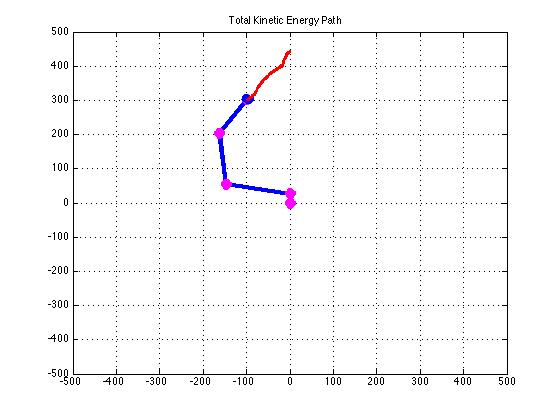
\includegraphics[scale=.135]{PathPics/Energy_Kinetic_Path.jpg}
\caption{Total Kinetic Energy Path}
\end{subfigure}

\caption{Paths When Considering Kinetic Energy}
\label{fig:EnergyPaths2}
\end{figure}
\end{frame}

\section{Conclusion}
\begin{frame}{Future Work}
\begin{itemize}
\item Consider other metrics\\
\begin{itemize}
\item Better angular kinetic energy metric
\item More accurate physics model of the arm
\end{itemize}
\item Using the robot base as part of the path finding
\item Increasing the grid size for smoother path
\item Move beyond simulation to the actual robot
\item Collision detection and obstacle avoidance
\end{itemize}
\end{frame}
\end{document}